\section{Scelta del modello}
\subsection{Grafici diagnostici}
\textbf{Osservazione.} È opportuno considerare che, nella scelta del modello, si è tenuto conto della discreta correlazione lineare osservata tra alcune variabili predittive, in particolare tra \textbf{x4\_MP} e \textbf{x7\_PixDensity} (correlazione pari a 0.743). \\ 
   Un’alta correlazione tra predittori può infatti dar luogo a fenomeni di \emph{multicollinearità}, ossia a situazioni in cui alcune variabili esplicative risultano linearmente dipendenti o quasi dipendenti. Ciò comporta una riduzione del rango della matrice di (\emph{design}), con conseguenti stime instabili dei coefficienti, varianze elevate e difficoltà nell’interpretazione individuale degli effetti delle singole variabili.
   
Di seguito vengono mostrati i grafici diagnostici ottenuti sui cinque modelli.
\begin{figure}[H]
	\centering
	\begin{minipage}{0.48\textwidth}
		\centering
		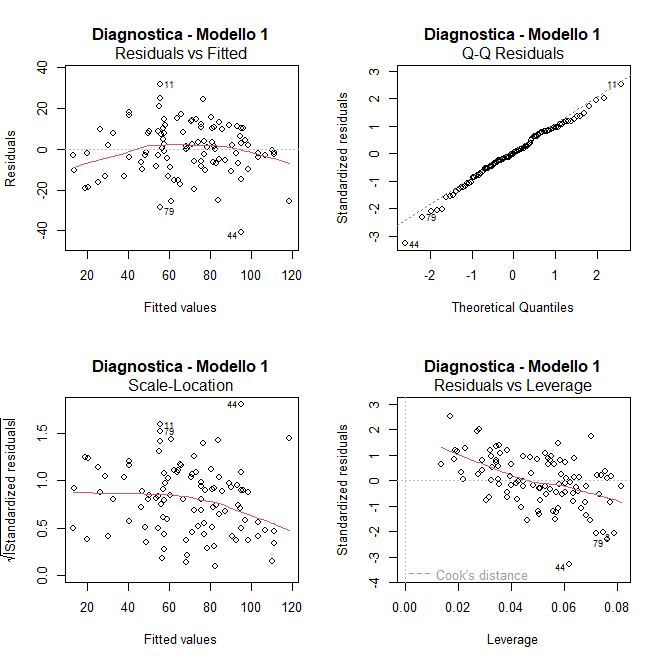
\includegraphics[width=\linewidth]{../graphs/diagnostica/modello1}
		\caption{Modello 1: diagnostica}
		\label{fig:diagnostica_modello1}
	\end{minipage}
	\hfill
	\begin{minipage}{0.48\textwidth}
		\centering
		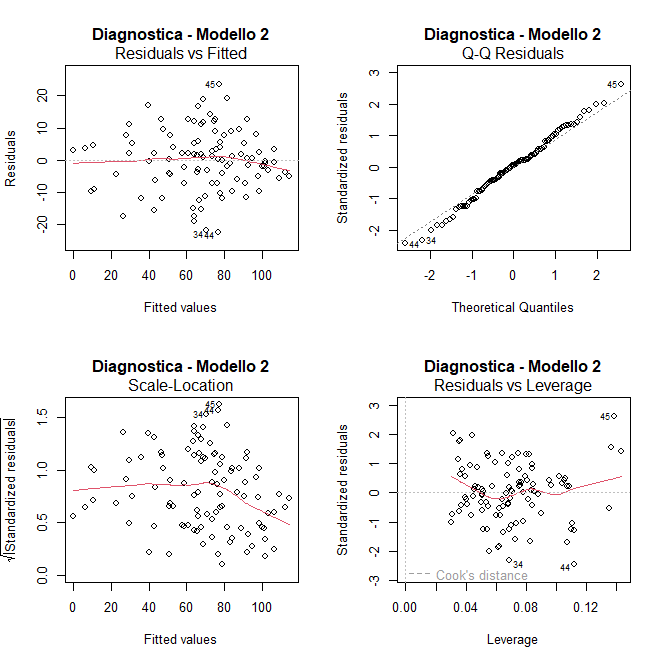
\includegraphics[width=\linewidth]{../graphs/diagnostica/modello2}
		\caption{Modello 2: diagnostica}
		\label{fig:diagnostica_modello2}
	\end{minipage}
\end{figure}

\begin{figure}[H]
	\centering
	\begin{minipage}{0.48\textwidth}
		\centering
		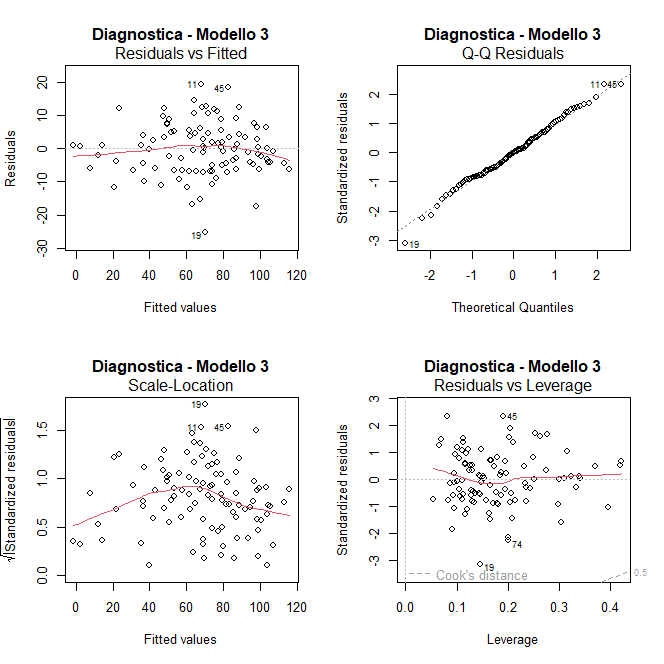
\includegraphics[width=\linewidth]{../graphs/diagnostica/modello3}
		\caption{Modello 3: diagnostica}
		\label{fig:diagnostica_modello3}
	\end{minipage}
	\hfill
	\begin{minipage}{0.48\textwidth}
		\centering
		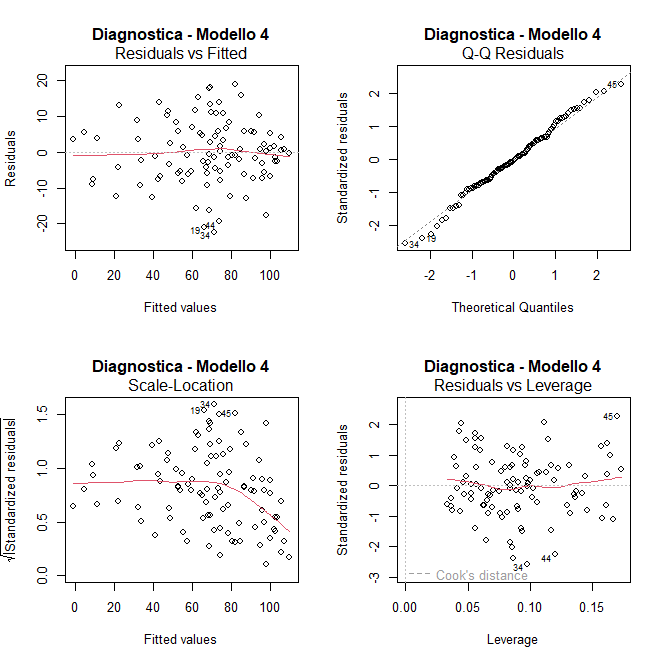
\includegraphics[width=\linewidth]{../graphs/diagnostica/modello4}
		\caption{Modello 4: diagnostica}
		\label{fig:diagnostica_modello4}
	\end{minipage}
\end{figure}

\begin{figure}[H]
	\centering
	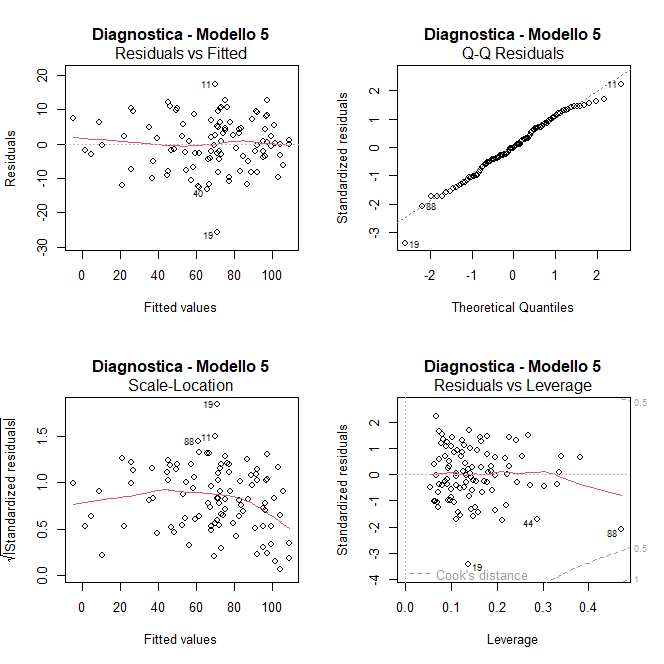
\includegraphics[width=0.75\linewidth]{../graphs/diagnostica/modello5}
	\caption{Modello 5: diagnostica}
	\label{fig:diagnostica_modello5}
\end{figure}

\subsection{Analisi dei parametri e verifica delle ipotesi classiche}
Si riportano i valori di $R^2$, AIC e MSE dei cinque modelli.
\begin{table}[H]
	\centering
	\begin{tabular}{|c|c|c|c|}
		\hline
		\textbf{Modello} & \textbf{adjusted} \boldmath$R^2$ & \textbf{AIC} & \textbf{MSE}\\
		\hline
		1 &  0.77  & 514.69 & 155.54\\
		2 & 0.87 & 460.76 & 87.16\\
		3 & 0.89 & 448.27 & 61.72\\
		4 & 0.88 & 451.67 & 76.45\\
		5 & 0.91 & 431.91 & 55.65 \\
		\hline
	\end{tabular}
	\caption{Valori di $R^2$ e AIC per i cinque modelli}
\end{table}
\begin{table}[H]
	\centering
	\begin{tabular}{|c|c|c|}
		\hline
		\textbf{Modello} & \textbf{W} & \textbf{p-value} \\
		\hline
		1 & 0.98908 & 0.5911 \\
		2 & 0.99307 & 0.8924 \\
		3 & 0.98997 & 0.6620 \\
		4 & 0.99147 & 0.7819 \\
		5 & 0.98235 & 0.2017 \\
		\hline
	\end{tabular}
	\caption{Esiti test di normalità tramite il test di Shapiro}
	\label{tab:coef_estimates}
\end{table}
\begin{itemize}
	\item \textbf{Linearità del modello:} Tra i modelli proposti, quello che meglio soddisfa quest'ipotesi è il modello 4. Infatti i valori si distribuiscono meglio intorno alla retta $y=0$.
	\item \textbf{Omoschedasticità:} In questo caso, osservando il grafico 'Scale-Location' il modello che meglio soddisfa l'ipotesi di varianza costante è il 4. Infatti è in questo modello che la nuvola di punti si distribuisce intorno all'ascissa.
	\item \textbf{Normalità dei residui: } Osservando i 'Q-Q Residuals' e gli esiti dei test di Shapiro sui residui, tutti i modelli soddisfano in buona maniera quest'ipotesi.
	\item \textbf{adjusted $R^2$, AIC, MSE:} Il modello 5, presenta i valori più piccoli di questi parametri, anche se i modelli 3 e 4 non si discostano troppo da questi valori. 
\end{itemize}
\subsection{Conclusioni}
A fronte dei dati ricavati e delle osservazioni fatte sulle ipotesi si stima che il modello che meglio descrive il dataset fornito è il modello 4. Infatti questo modello fra tutti meglio soddisfa le ipotesi classiche e inoltre riesce a spiegare molto bene la variabilità del dataset senza essere troppo legato allo specifico dataset. 


